\documentclass[final]{beamer}
% \usecolortheme{crane}
\mode<presentation>
{
  \usetheme{I6pd2}
}
\usepackage{times}
\usepackage{amsmath,amssymb}
%\usepackage{sfmath} % for sans serif math fonts; wget http://dtrx.de/od/tex/sfmath.sty
\usepackage[english]{babel}
\usepackage[utf8]{inputenc}
\usepackage[size=a4, scale=0.4]{beamerposter}
\usepackage{booktabs,array}
\usepackage{wrapfig}
% \usepackage{enumitem}

% Display a grid to help align images
% \beamertemplategridbackground[3mm]

\title{\LARGE Algorithmic Analysis of Code-Breaking Games}

\author{Mgr. Miroslav Klimoš, prof. RNDr. Antonín Kučera Ph.D.}
\institute[]{ Faculty of Informatics, Masaryk University, Brno }

\date[May. 28th, 2008]{May. 28th, 2008}

\newcommand{\thando}[4]{
\begin{columns}[T]
\begin{column}{\leftmarginii}
\end{column}
\begin{column}{#3\textwidth}
\vspace{-1.5mm}
\begin{itemize}
#1
\end{itemize}
\end{column}
\begin{column}{#4\textwidth}
#2
\end{column}
\end{columns}\medskip}

\setbeamersize{text margin left=8mm,text margin right=8mm}

\begin{document}

\begin{frame}{} 
\begin{columns}[t, totalwidth=\textwidth]
  %%%%%%%%%%%%%%%%%%%%%%%%%%%%%%%%%%%%%%%%%%%%%%%%%%%%%%%%%%%%%%%%%%%%%%%%%%%%%%%%%%%%%%%%%%%%%%%%%%%%
  %%%%%%%%%%%%%%%%%%%%%%%%%%%%%%%%%%%%%%%%%%%%%%%%%%%%%%%%%%%%%%%%%%%%%%%%%%%%%%%%%%%%%%%%%%%%%%%%%%%%
  \begin{column}{.485\textwidth}
    
    \begin{block}{Code-Breaking Games}
      \begin{itemize}
      \item 2 players: \emph{codemaker} and \emph{codebreaker}
      \item Codemaker selects a \emph{secret code}
      \item Codebreaker strives to reveal the code through a series of \emph{experiments} whose outcomes give partial information about the code
    \vskip1ex
    \item Example: Mastermind
    \vskip-2.5ex
    \begin{columns}
      \begin{column}{12mm}\end{column}
      \begin{column}{.78\textwidth}
        \begin{itemize}
        \item Secret code: combination of $n$ \emph{coloured pegs}
        \item Codebreaker makes guesses (experiments)
        \item Guesses are evaluated with \emph{black and white markers}
        \item Black marker = correct both colour and position
        \item White marker = the colour is present at a different position
        \end{itemize}
      \end{column}

      \begin{column}{.22\textwidth}
        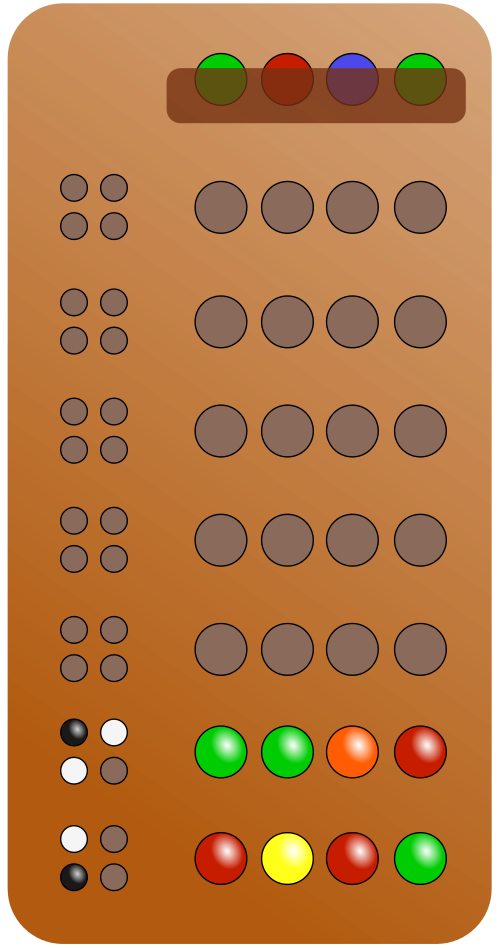
\includegraphics[width=1.8cm]{../pictures/mastermind.png}
      \end{column}
    \end{columns}
    \item Example: Counterfeit Coin
      \begin{columns}
      \begin{column}{10mm}\end{column}
      \begin{column}{\textwidth}
        \begin{itemize}
        \item Problem of finding an odd-weight coin using balance scale
        \item Secret code: identity of the unique counterfeit coin 
        \item Codebreaker puts coins on the balance scale and observes the outcome %(the left pan is lighter / heavier / same)
        \end{itemize}    
      % \end{column}
      % \begin{column}{.22\textwidth}
      %   % 
\includegraphics[width=2cm]{../pictures/scales.pdf}
      \end{column}
      \end{columns}
    \end{itemize}
    \end{block}
      
  \end{column}\hspace{4.2mm}~
  %%%%%%%%%%%%%%%%%%%%%%%%%%%%%%%%%%%%%%%%%%%%%%%%%%%%%%%%%%%%%%%%%%%%%%%%%%%%%%%%%%%%%%%%%%%%%%%%%%%%
  %%%%%%%%%%%%%%%%%%%%%%%%%%%%%%%%%%%%%%%%%%%%%%%%%%%%%%%%%%%%%%%%%%%%%%%%%%%%%%%%%%%%%%%%%%%%%%%%%%%%
  \begin{column}{.485\textwidth}

    \begin{block}{Questions and Problems}
      \medskip
      \begin{quote}
      How should the codebreaker play in order to minimize the number of~experiments needed to undoubtedly determine the code?
      \end{quote}
      \begin{quote}
      Is there a strategy for experiment selection that guarantees revealing the~code after at most $k$ experiments?
      \end{quote}
      \begin{quote}
      What strategy is optimal with respect to the average-case number of~experiments, given that the code is selected from the given set with uniform distribution?
      \end{quote}

      \begin{itemize}
      \item We create a computer program to automatically answer these questions
      \end{itemize}
      \vskip1.1ex
      \hspace{5mm}\begin{picture}(280,80)
      \put(30,30){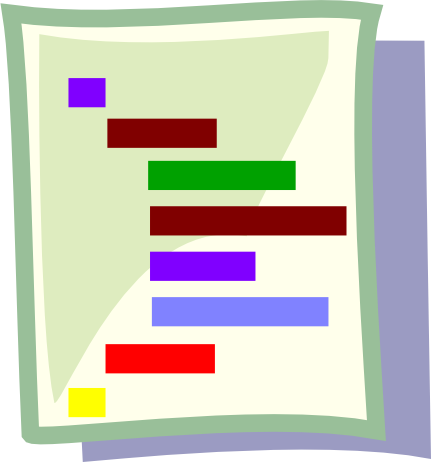
\includegraphics[width=15mm]{spec.png}}
      \put(130,28){
\includegraphics[width=16mm]{gears.png}}
      \thicklines
      \put(80,50){\vector(1,0){40}}
      \put(0,10){\parbox{3.5cm}{\centering specification of \\a code-breaking game}}
      \put(125,10){\parbox{2cm}{\centering computer \\program}}
      \put(185,50){\vector(2,1){40}}
      \put(185,50){\vector(2,0){40}}
      \put(185,50){\vector(2,-1){40}}
      \put(235,20){\parbox{5cm}{bounds on number \\of experiments}}
      \put(235,45){\parbox{5cm}{value of a given strategy}}
      \put(235,67){\parbox{5cm}{optimal strategy}}
      \end{picture}
    \end{block}

  \end{column}
  \end{columns}

    \vskip2.2ex
    \begin{block}{Steps Towards Automatic Analysis}
      \begin{columns}[T]
      \begin{column}{0.48\textwidth}
      \begin{enumerate}
      \item Creating a general, formal model of code-breaking games
        \thando{
        \item Model based on propositional logic
        \item Secret code = valuation of variables
        \item Partial information = logical formula
        }{
          % \hspace{-12mm}
          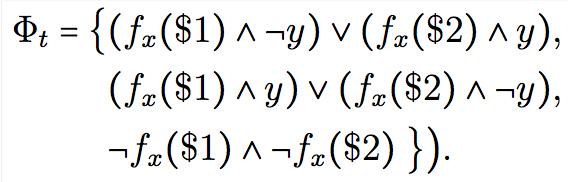
\includegraphics[scale=0.45]{img-model.png}
        }{0.65}{0.35}
      \item Proposing general strategies for experiment selection
        \thando{
        \item \emph{``Select an experiment that minimizes the maximal\\ number of possibilities for the code in the next round''}
        \item Several strategies of this kind formalized within the~model
        }{
          \vskip-2ex
          \hspace{-8mm}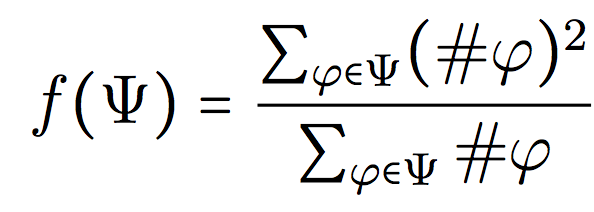
\includegraphics[width=3cm]{img-strategy.png}
        }{0.8}{0.2}
      \item Developing algorithms for strategy evaluation and synthesis
        \thando{
        \item Based on intelligent backtracking
        \item Symmetry detection reduces the size of the state-space
        }{
          \vskip-5ex
          \hspace{-8mm}
          ~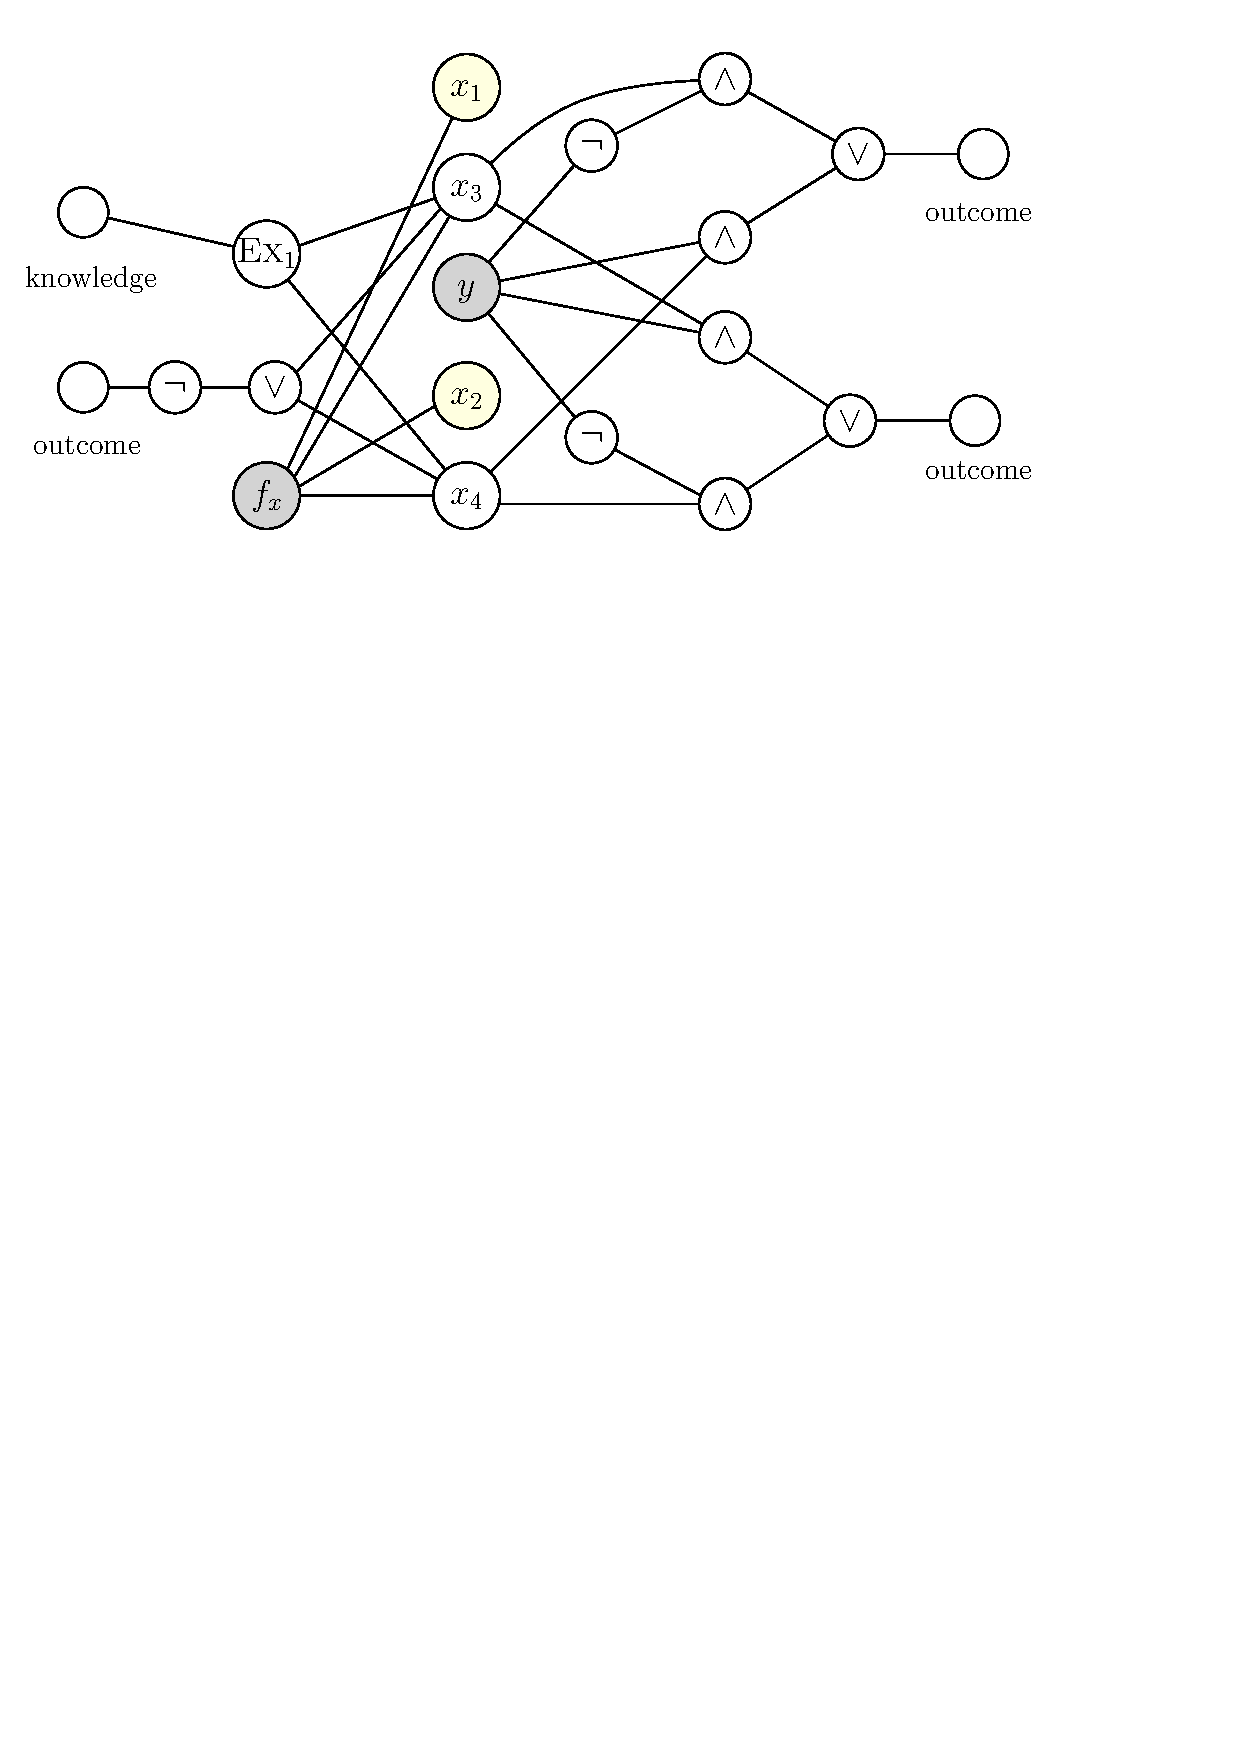
\includegraphics[width=4cm]{../pictures/exp-graph-sim.pdf}
        }{0.75}{0.25}
      \end{enumerate}
      \end{column}
      \begin{column}{0.48\textwidth}
      \begin{enumerate}
      \item[4.] Designing a computer language for game specification
        \thando{
        \item Corresponds to the formal model
        \item Built on top of Python for easier generation
        }{
          \hspace{-17mm}
          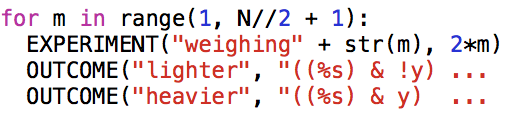
\includegraphics[width=4cm]{img-language.png}
        }{0.75}{0.25}
      \item[5.] Implementing proposed algorithms in a computer program
        \thando{
        \item Command-line tool written in C++
        \item Use of modern SAT solvers for satisfiability queries needed by the algorithms
        % \item Graph canonization tool Bliss utilized for symmetry detection
        }{

        }{0.95}{0.05}
      \item[6.] Using the program to create new and reproduce existing results
        \thando{
        \item Easy reproduction of some of the existing results for~Mastermind
        \item Automatic analysis of generalizations and \\other code-breaking games
        }{
          % \hspace{-5mm}
          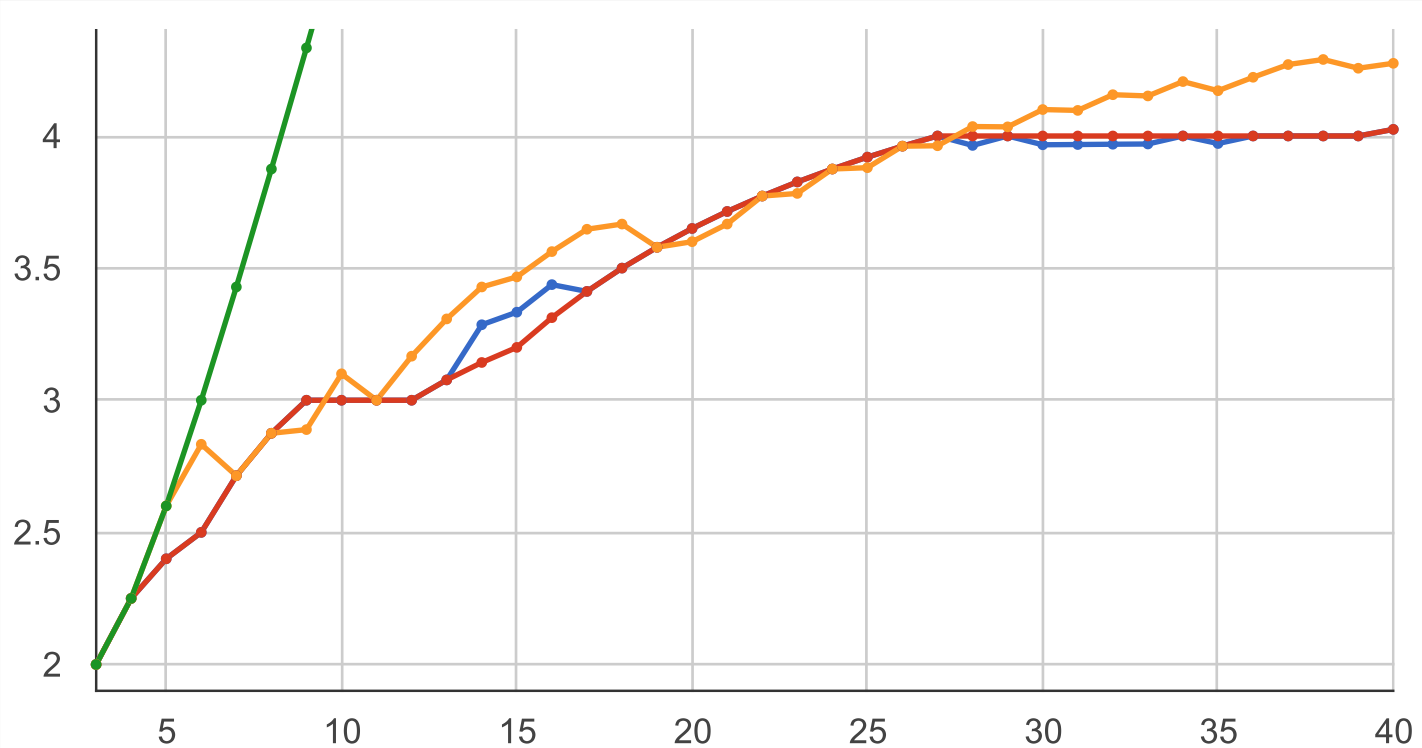
\includegraphics[width=4.5cm]{img-results.png}
        }{0.6}{0.4}
        \end{enumerate}
        \vspace{-3ex}~
      \end{column}
      \end{columns}
    \end{block}       
  % \end{column}
  %%%%%%%%%%%%%%%%%%%%%%%%%%%%%%%%%%%%%%%%%%%%%%%%%%%%%%%%%%%%%%%%%%%%%%%%%%%%%%%%%%%%%%%%%%%%%%%%%%%%
  %%%%%%%%%%%%%%%%%%%%%%%%%%%%%%%%%%%%%%%%%%%%%%%%%%%%%%%%%%%%%%%%%%%%%%%%%%%%%%%%%%%%%%%%%%%%%%%%%%%%
% \end{columns}
\vfill
\end{frame}

\end{document}
%%%%%%%%%%%%%%%%%%%% 
%%% Local Variables: 
%%% mode: latex 
%%% TeX-PDF-mode: t 
%%% End: 
